\section{Experiments}
\subsection{Naive Feed-forward Deep Neural Networks}

What we call our Naive Feed-forward network is the benchmark we made to test the efficacy of the models we were training. We tested several versions before deciding on a final candidate Naive Model. We had a categorical classifier, a regression model, and another categorical model with a better layer design.

\subsubsection{Naive Categorical Model} 

Our first model had inputs of one hots for movies and users, mean, median and variance of the current movie calculated from the training set, and time represented as a month input, a day input, and a year since beginning input. This model had two hidden layers with 128 nodes each using relu activation and a softmax output to guess categorically what the rating was for that user. With this configuration the model converged to about 38\% accuracy on our validation set. Because of the distribution of ratings in our data set this is about as good as always guessing the rating 4 for every movie. Not great, but better than randomly chance.

\subsubsection{Naive Regression Model}

For training the problem as a regression model we learned we had to be very careful with the layer selection. Too few layers and inadequate funneling down of the layers towards the output layer resulted in a model that was hopelessly lost at trying to find a gradient. We finally had success with a model using a hidden layers of size 512, 64, 8, and a linear output layer. After training we were surprised  because it had a very good RMSE score. Closer inspection showed that the model was predicting a floating point value that was always between 3.4 and 3.6, very close to the mean value of the data set. When we rounded the value and calculated the accuracy and RMSE it was only 21\% accurate with and RMSE of 1.203.

\subsection{Neural Network Embeddings on the Netflix Dataset}
Since it was unclear how, or whether, to attempt to model ratings in the latent space, several experiments were carried out on both the movie embeddings and user embeddings over the Netflix dataset:
\begin{itemize}
\item User Embeddings trained as CBOW across all rating events
\item User Embeddings trained as CBOW across positive (>3 rating) rating events
\item User Embeddings computed as a weighted mean of all movie embeddings for movies that a user has watched
\item Movie Embeddings trained as CBOW across all rating events
\item Movie Embeddings trained as CBOW across positive (>3 rating) rating events
\item Movie Embeddings computed as a weighted mean of all user embeddings for movies that a user has watched
\end{itemize}

\subsection{Neural Network Embeddings on the IMDB Dataset}
A principle contributor neural network embedding layer was built using CBOW training - treating the context for a principle as the other principles that had worked in conjunction with the target on a movie. The embedding dimension was 64, and this model was trained using noise contrastive error as loss for 500 epochs to a loss of 5.23. Movies embeddings were then computed as the mean of their constituent principle embeddings. 
\begin{figure}[h]
    \centering
    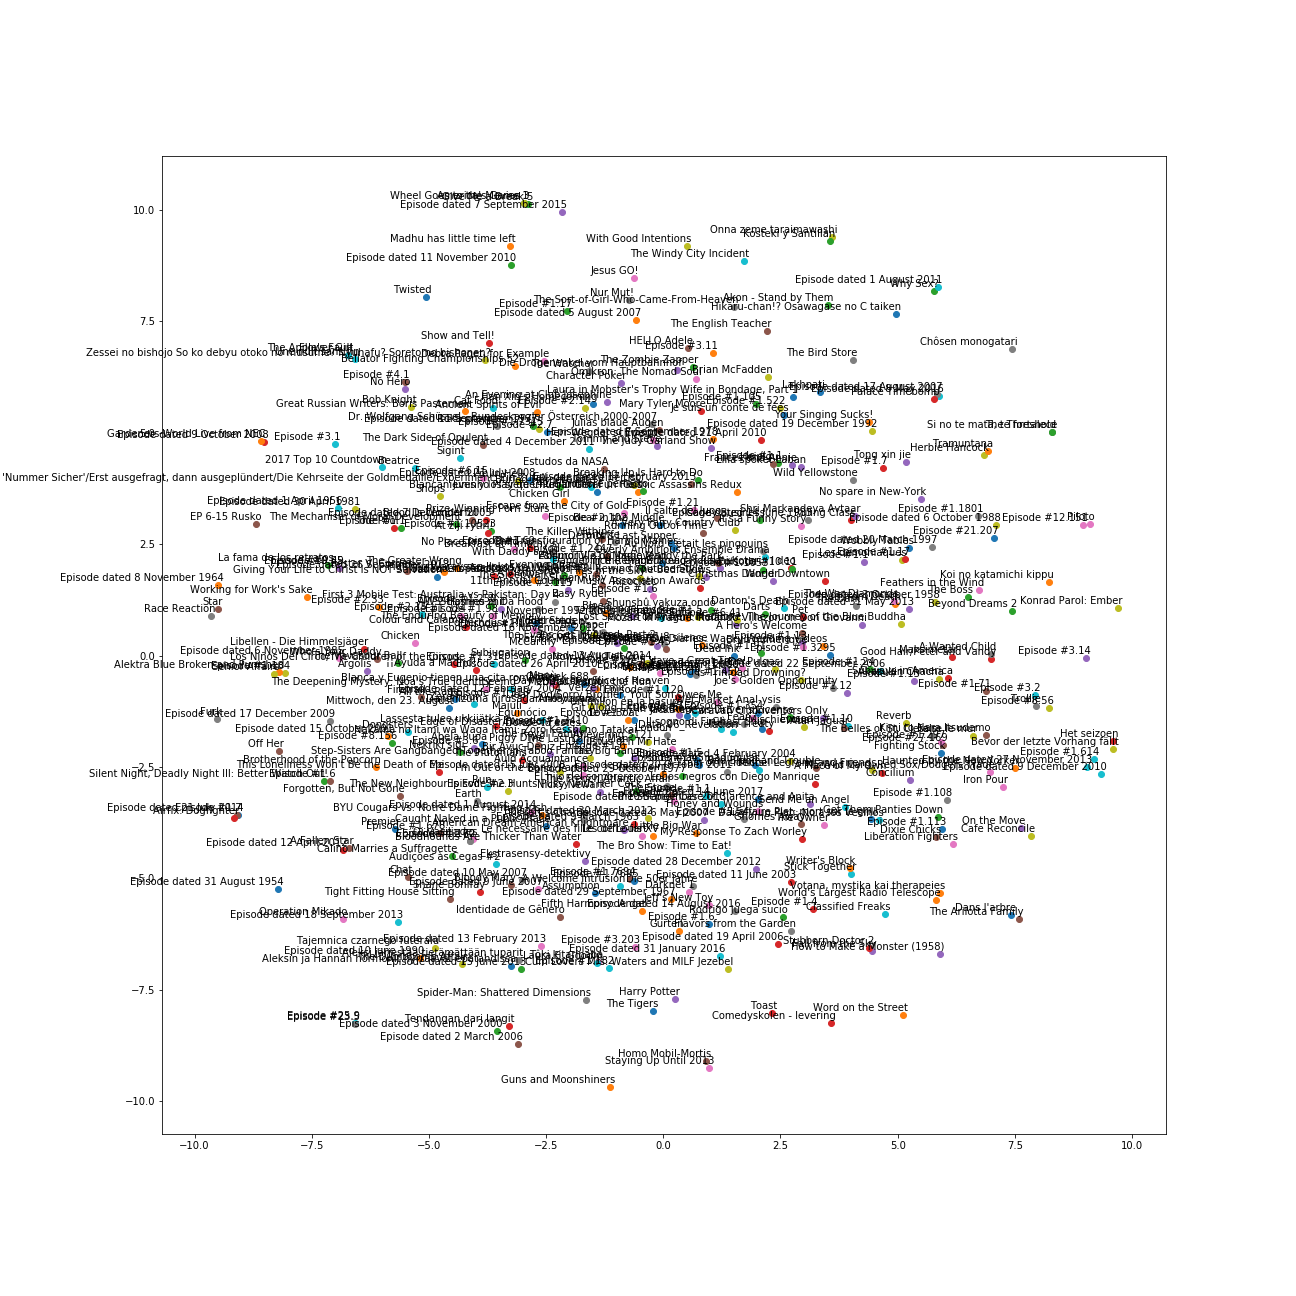
\includegraphics[width=0.45\textwidth]{images/imdb_movie_embeddings_100.png}
    \caption{TSNE Visualization of Embeddings for 100 Movies in the IMDB Movie Catalog}
    \label{fig:TSNE IMDB Movie Embeddings}
\end{figure}
Since the Netflix and IMDB movie catalogs had significant overlap, but neither were a subset of the other, multitask training was planned to form a joint embedding space merging the features of both embeddings. Unfortunately due to time constraints, this could not be finished.
\subsection{SVD Embeddings on the Netflix Dataset}

In \cite{He2017} they use a process the call GMF or Generalized Matrix Factorization where they use gradient descent to train their embedding to learn the most important latent features

When considering the methods for representing User and Movie matrix factorization embeddings, we decided on using Single Value Decomposition, primarily because it is implemented in the scipy package, and could operate on sparse matrices. This was important because the original matrix we would be decomposing would be of size 440,000 x 17776 and would not possibly fit into memory. 

\subsection{Deep Feed-forward Neural Networks with Embedding Layers}

\subsubsection{SVD Deep Embeddings}
We needed some way to evaluate how useful the information presented by the SVD Embeddings would be to a deep learning model. We decided to train models on combinations of embeddings and one hots only, without other contextual information like, date of review, actor, genre, etc to see how useful these representations would be. This would tell us, given only a representation of likeness to other users we had computed, how well we could predict their tastes. If we could beat the threshold of randomly guessing or always rating 4, the marks set by our benchmark naive model, than the matrix factorization embeddings would be considered a success.

To test this we first trained to convergence a model that took as inputs both the User SVD embedding and a one hot for its movie id. It was during training this model we experimented with adding more layers and funneling their output as mentioned in \cite{He2017} with hidden layers of our input size (17826), 1000, 100, 10, and a softmax output layer we were able to achieve an accuracy of around 42\%

We also tested using both the User SVD and the Movie SVD as the inputs. This would shrink the input size down from 17826 to 125. Training a model that again had 4 hidden layers we were able to reach an accuracy of 45\%. Clearly the representations did have value.

Unfortunately we were not able to also train a model using user one hots and movie embeddings, as the input size made computation prohibitively dificult. 



\subsection{Hierarchical Architectures}
